\chapter{Marco Procedimental}
\par Para realizar exitosamente un proyecto de desarrollo de software, es necesario escoger un método y establecer un plan de trabajo con el fin de organizar el flujo de las actividades, definir las metas y sus lapsos de tiempo de ejecución, en otras palabras, establecer una metodología de desarrollo que posibilite completar las tareas correspondientes eficientemente. \\
\par Una metodología de desarrollo de software puede ser definido como un conjunto estandarizado de conceptos, prácticas y criterios con la finalidad de estructurar, planear y controlar un proceso de desarrollo de software de calidad, a menudo ella es vinculada a algún tipo de organización, la cual promueve su uso y hace los refinamientos requeridos. A continuación, se procederá a explicar brevemente las metodologías mas utilizadas para el desarrollo de software.

\section{Metodologías Tradicionales}
\par Las metodologías Tradicionales refieren a la forma ``tradicional'' de desarrollar un software. Ellas se basan en seguir una serie secuencial de pasos, tales como definición de requisitos, creación de soluciones, pruebas e implementación. Estos requisitos deben ser definidos y documentados al comienzo del proyecto.\\
\par  Debido a estos requisitos y aspectos, estas metodologías tradicionales también son conocidas como metodologías ``pesadas''. Algunos profesionales encontraron frustrante esta visión centrada en el proceso del desarrollo de software y reportan dificultades aún cuando las tasas de cambio son relativamente bajas. Las metodologías pesadas tienen las siguientes características similares \cite{BOOK08}:
\begin{itemize}
    \item Enfoque predictivo: las metodologías pesadas tienden a primero planificar en detalle gran parte del proceso, consumiendo un largo periodo de tiempo. Este enfoque sigue una disciplina de ingeniería donde el desarrollo es predictivo y repetible. Se pone mucho énfasis en los diagramas, enfocándose en la necesidad del sistema y en cómo resolver las necesidades de manera eficiente.
    \item Documentación integral: el desarrollo de software tradicional, considera el documento de requisitos como la pieza clave de la documentación. Un proceso principal en las metodologías pesadas, es el largo proceso inicial de diseño, en el que se considera, que es posible reunir todos los requisitos por adelantado, antes de escribir cualquier código.
    \item Orientado a procesos: el objetivo de las metodologías pesadas es definir un proceso que funcione bien. El proceso consistirá en ciertas tareas que deben realizar los gerentes, diseñadores, programadores, testers, otros.
    \item Orientado a herramientas: las herramientas de gestión de proyectos, editores de código, compiladores y otras, se deben utilizar para completar y entregar cada tarea.
\end{itemize}

\section{Metodologías Ágiles}
\par En las metodologías tradicionales, no se toma en cuenta el factor humano en el desarrollo de software, así como tampoco se hace énfasis en los problemas y cambios que pueden surgir a lo largo del proyecto, por este motivo nace el término ``ágil'' aplicado al desarrollo de software. El objetivo principal de las metodologías ágiles, es destacar un nuevo grupo de valores y principios, que permitieran dar respuesta rápida a los problemas surgidos durante el desarrollo. \\
\par \textit{The Agile Alliance} es una organización sin fines de lucro, dedicada a promover los conceptos relacionados con el desarrollo ágil del software, su punto de partida fue el Manifiesto Ágil, un documento que resume su filosofía y plantea los siguientes principios \cite{BOOK06,BOOK07}:
\begin{itemize}
    \item   La mayor prioridad es satisfacer al cliente, mediante la temprana y continua entrega de software de calidad.
    \item	Los cambios en los requerimientos son bienvenidos, incluso en fases tardías del desarrollo.
    \item	Entregas frecuentes de software funcional, en intervalos de dos semanas a dos meses, dando preferencia a los tiempos más cortos.
    \item	Los clientes y los desarrolladores deben trabajar diariamente y en conjunto a lo largo del proyecto.
    \item	Construir proyectos alrededor de individuos motivados. Darles el ambiente y el apoyo que necesitan y confiar que realizarán el trabajo de manera correcta.
    \item	El método más eficiente y efectivo de comunicación entre los miembros del equipo de trabajo es la conversación cara a cara.
    \item	La principal métrica del progreso es que el software funcione correctamente.
    \item	Los procesos ágiles promueven un desarrollo sostenible.
    \item	Atención continua a la excelencia y el buen diseño.
    \item	La simplicidad es esencial.
    \item	Las mejores arquitecturas, requerimientos y diseños surgen de equipos de trabajo organizados por sí mismos.
    \item	El equipo analiza cómo ser más efectivo y adecua su comportamiento al resultado de discusiones realizadas regularmente. 

\end{itemize}
\subsection{Scrum}

\par Scrum es un modelo referencial, define un conjunto de prácticas, roles y el punto de partida para la creación del proceso a ejecutar según la duración del proyecto \cite{BOOK11}. \\

\par Scrum no requiere ni proporciona métodos/prácticas de desarrollo de software específicos para ser utilizados. En cambio, requiere ciertas prácticas y herramientas de gestión en diferentes fases de Scrum, para evitar el caos por impredecibilidad y complejidad.
\subsubsection{Prácticas Principales}
\begin{itemize}
    \item Backlog del Producto: es la lista priorizada de todas las características y cambios que aún deben realizarse en el sistema, requerido por múltiples actores.
    \item Sprints: Las herramientas de gerencias del equipo son las reuniones de planificación de Sprint, la revisión del Sprint y las reuniones diarias de Scrum.
    \item Reunión de planificación de Sprint.
    \item Sprint Backlog: es la lista de funciones que realmente se asigna a un Sprint en particular. 
    \item Scrum diario: es una reunión diaria de aproximadamente 15 minutos. 
\end{itemize}

\par El proceso Scrum puede cambiar considerablemente la descripción del trabajo y las costumbres del equipo del proyecto Scrum \cite{BOOK08,BOOK11}.
%%%%%%%%%%%%%%%

\subsection{XP: \textit{Extreme Programming}}

\par El proceso XP se caracteriza por ciclos cortos de desarrollo, planificación incremental, retroalimentación continua, dependencia de la comunicación y diseño evolutivo \cite{BOOK10}. Los miembros del equipo XP dedican muchas veces al día unos minutos a la programación, unos a la gestión del proyecto, otros al diseño, a la retroalimentación y al trabajo en equipo \cite{BOOK09}. A continuación se muestra un resumen de los términos y prácticas de XP \cite{BOOK09,BOOK10}:
\begin{itemize}
    \item \textbf{Planificación:} el programador estima el esfuerzo necesario para la implementación, el cliente decide el alcance y el momento de los lanzamientos en función de las estimaciones.
    \item \textbf{Lanzamientos cortos:} la aplicación se desarrolla en una serie de versiones pequeñas y frecuentemente actualizadas. Se lanzan nuevas versiones en frecuencia desde diario a mensual.
    \item \textbf{Diseño simple:} el énfasis está en el diseño de la solución más simple posible. La complejidad innecesaria y el código adicional se eliminan de inmediato.
    \item \textbf{Metáfora:} el sistema se define mediante un conjunto de metáforas entre el cliente y los programadores, que describen cómo funciona el sistema.
    \item \textbf{Refactorizar:} implica la reestructuración del sistema simplificándolo, eliminando la duplicación, mejorando la comunicación y agregando flexibilidad.
    \item \textbf{Programación en pares:} todo el código de producción lo realizan dos programadores en una computadora.
    \item \textbf{Integración continua:} todo código nuevo se integra con el sistema tan pronto como esté listo. Al integrarse, el sistema se construye nuevamente y los cambios son aceptados una vez que pasan todas las pruebas.
    \item \textbf{Cliente en el sitio:} el cliente debe estar disponible en todo momento con el equipo de desarrollo.
    \item \textbf{Estándares de codificación:} existen reglas para la escritura de todo código y los desarrolladores las siguen para brindar consistencia y mejorar la comunicación entre el equipo de desarrollo.
\end{itemize}

\par El ciclo de vida de un proyecto XP se divide en seis fases: exploración, planificación, iteraciones para el lanzamiento, producción, mantenimiento y muerte, Ver figura \ref{fig:xp01}. 

\begin{figure}[htpb!]
	\centering
	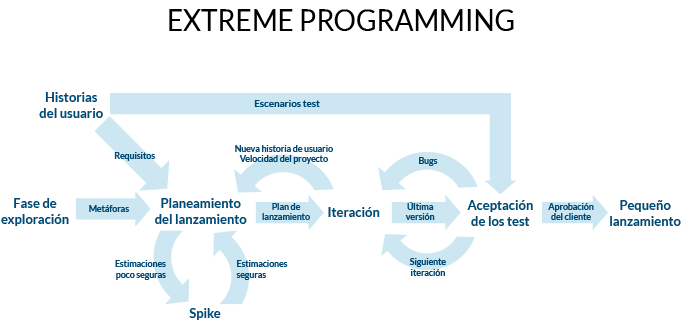
\includegraphics[width=0.91\columnwidth]{images/xp01.png}
	\caption{Ciclo de vida de XP.}
	\label{fig:xp01}
\end{figure}

\subsection{Kanban}

\par El enfoque Kanban es una de las adiciones más reciente al desarrollo de software ágil, pero fue introducida por la industria Japonesa en el año 1950. El método Kanban en el desarrollo de software se originó en 2004 y se basa en impulsar a los equipos de proyectos a visualizar el flujo de trabajo, limitar el trabajo en progreso (WIP o Work In Progress por sus siglas en ingles) en cada etapa del flujo de trabajo y medir el tiempo del ciclo \cite{LIB22}.\\ 

\par Kanban se basa en el uso de un tablero o panel llamado tabla Kanban  (Ver \ref{fig:xp01}), que  proporciona visibilidad al proceso de software, porque muestra el trabajo asignado a cada desarrollador, comunica claramente las prioridades y destaca los cuellos de botella. Además, su objetivo es minimizar el WIP, es decir, desarrollar solo los elementos que se solicitan. Esto produce un flujo constante de elementos de trabajo liberados a los clientes, ya que los desarrolladores se centran solo en esos pocos elementos en un momento dado. El método Kanban tiene como objetivo adaptar rápidamente el proceso mediante el uso de ciclos de retroalimentación más cortos \cite{LIB22}.\\

\par Los siguientes son los principios básicos de Kanban, los cuales son necesarios resaltados en el tablero, para el desarrollo de software son \cite{LIB23}:
\begin{itemize}
    \item Limitación del trabajo en proceso (WIP).
    \item Tirando valor a través del proceso de desarrollo.
    \item Hacer visible el proceso de desarrollo.
    \item Aumento del rendimiento.
    \item Utilizando un listado de tareas fijo (tablero).
    \item Calidad de acoplamiento.
\end{itemize}

\begin{figure}[htpb!]
	\centering
	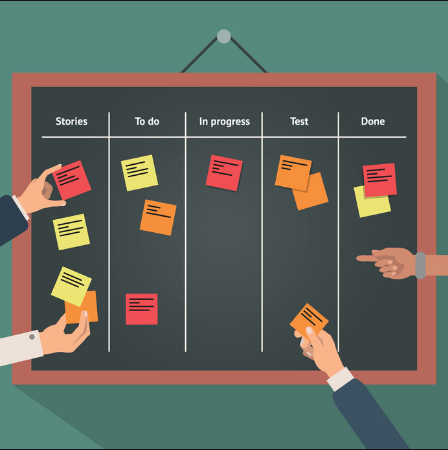
\includegraphics[width=0.875\columnwidth]{images/kanban01.PNG}
	\caption{Tablero Kanban.}
	\label{fig:kanban01}
\end{figure}

\par La metodología Kanban se enfoca en hacer el trabajo correcto en el momento adecuado, dados los conjuntos de habilidades de los desarrolladores y velocidades de trabajo. Estos comienzan implementando componentes del proyecto que agregan valor al proyecto. También se evita implementar funciones innecesarias, escribir más especificaciones de las que puedan codificar y  código del que pueda probar, para no probar mas código del que se pueda implementar. Por esto Kanban elimina cualquier desperdicio en cada paso \cite{LIB23}.
